% This is samplepaper.tex, a sample chapter demonstrating the
% LLNCS macro package for Springer Computer Science proceedings;
% Version 2.21 of 2022/01/12
%
\documentclass[runningheads]{llncs}
%
\usepackage[T1]{fontenc}
% T1 fonts will be used to generate the final print and online PDFs,
% so please use T1 fonts in your manuscript whenever possible.
% Other font encondings may result in incorrect characters.
%
\usepackage{graphicx}
% Used for displaying a sample figure. If possible, figure files should
% be included in EPS format.
%
% If you use the hyperref package, please uncomment the following two lines
% to display URLs in blue roman font according to Springer's eBook style:
%\usepackage{color}
%\renewcommand\UrlFont{\color{blue}\rmfamily}
%\urlstyle{rm}
%


%  Ed added the following packages %%%%%%%%%%%%%%%%%%%%%%%%%%
\usepackage{url}
%\def\UrlFont{\rmfamily}
\usepackage{graphicx}
\usepackage{amsmath}
\usepackage{epstopdf}% To incorporate .eps illustrations using PDFLaTeX, etc.
%\usepackage[caption=false]{subfig}% Support for small, `sub' figures and tables
%\usepackage[square,sort,comma,numbers]{natbib}

%\usepackage{fix-cm}
\usepackage{graphicx}  
\usepackage[hidelinks]{hyperref}  % for including hyperlinks in document, the hidelinks removes the green box in the pdf
%\usepackage{listings} % for source code listing
%\usepackage{color} % for source code listing

\usepackage{nccmath}
\usepackage{amssymb}% http://ctan.org/pkg/amssymb
%\usepackage{pifont}% http://ctan.org/pkg/pifont

%\usepackage{microtype} % relaxes the rules for inter word spacing 
%\usepackage[T1]{fontenc}
%\usepackage{lmodern}

\usepackage{tabularray}   % for table 
\usepackage{multirow}     % for centering content in a table 
%\usepackage{array, booktabs, ragged2e}
%\newcolumntype{P}[1]{>{\centering\arraybackslash}p{#1}}
%\newcolumntype{M}[1]{>{\centering\arraybackslash}m{#1}}

% Change the title of the Bibliography to References and make it left-justified
%\renewcommand{\bibname}{References}
%\makeatletter
%\renewcommand\bibsection{
	%	\section*{\refname\@mkboth{\MakeUppercase{\refname}}{\MakeUppercase{\refname}}}
	%}
%\makeatother

% Change the title of the Bibliography to References
%\def\bibname{References}

\usepackage{graphicx}
\usepackage[table,xcdraw]{xcolor}
% Beamer presentation requires \usepackage{colortbl} instead of \usepackage[table,xcdraw]{xcolor}

% Ed Stopped adding packages here %%%%%%%%%%%%%%%%%%

\begin{document}
%
\title{Title of your paper here}
%
% If the paper title is too long for the running head, you can set
% an abbreviated paper title here
\titlerunning{Your running title here ....}
%
%
\author{First Author\inst{1}\orcidID{0000-1111-2222-3333} \and
Second Author\inst{2,3}\orcidID{1111-2222-3333-4444} \and
Third Author\inst{3}\orcidID{2222--3333-4444-5555}}
%
% First names are abbreviated in the running head.
% If there are more than two authors, 'et al.' is used.
\authorrunning{F. Author et al. -- replace this with the authors}
%
%
\institute{Princeton University, Princeton NJ 08544, USA \and
Springer Heidelberg, Tiergartenstr. 17, 69121 Heidelberg, Germany
\email{lncs@springer.com}\\
\url{http://www.springer.com/gp/computer-science/lncs} \and
ABC Institute, Rupert-Karls-University Heidelberg, Heidelberg, Germany\\
\email{\{abc,lncs\}@uni-heidelberg.de}}
%
\maketitle              % typeset the header of the contribution
%
%
\begin{abstract}
The abstract should briefly summarize the contents of the paper in
150--250 words.

\keywords{First keyword  \and Second keyword \and Another keyword.}
\end{abstract}
%
%
\section{Introduction}
\label{Introduction}

In the modern era, software has become ubiquitous in human life. It can be found in cell phones, computers, vehicles, etc. Due to technological advancements such as the internet, it has become more important for companies to rapidly iterate on and update their software products to keep up with changing requirements from customers, stay ahead of competitors and maintain security. The concept of continuous integration and continuous delivery (CI/CD) was created to aid in solving these issues by emphasizing rapid delivery of changes to customers via automation. Automated software testing is one important piece of CI/CD which is used to maintain high quality software and reduce the risk of software failures. However, typically as software increases in scale and complexity, running automated test suites can take several hours. This often hinders software engineers in their development lifecycle especially when errors are discovered. Each fix can take hours to validate before additional changes can be made, resulting in significant delays when releasing updates.

Typically, for CI/CD, companies use systems such as Jenkins, GitHub Actions or GitLab CI. While these technologies support the connection of multiple servers to handle several workloads simultaneously, often, automated test suites are executed on a single computer per pipeline. One potential solution is to increase the number of tests that can be run at the same time and the speed at which these tests are executed using Distributed Computing. Distributed Computing in this context refers to spreading workloads such as automated tests across several computers, potentially in different physical locations, to increase the amount of work that can be done in parallel. To that end, this paper seeks to answer to what extent can test execution leverage distributed computing to improve efficiency and speed, considering factors such as memory and CPU usage, execution time, the trade-offs between vertical and horizontal scaling, and cost-effectiveness at scale.

The remaining sections of this paper are as follows: The next section will provide some background information on distributed computing and using this strategy for testing. In Section~\ref{Methodology}, we describe the design of our solution and the methods we used to measure and compare our solution to traditional approaches. In the Section~\ref{Findings}, we will present the results of our quantitative analysis which will then be further analyzed in Section~\ref{Discussion}. Finally, Section~\ref{Conclusion} will conclude the paper and propose potential future paths that can be explored.
\section{Background}
\label{Background}

Replace all this with a relevant comprehensive literaure review in your specific area of interest in Software Testing.  The Background section provides context and detailed information needed to understand the research problem. It typically includes a review of existing literature, key concepts, theories, and previous studies relevant to the topic. The goal is to frame the research by outlining what is already known, identifying gaps in the knowledge, and explaining why the current study is necessary. The background helps the reader understand how the research fits into the broader field and what it aims to contribute. 

The rapid evolution of Generative AI has profoundly transformed technological capabilities, significantly influencing societal interactions, business processes, and educational methodologies. This section is divided into three main parts. The first part delves into the key technologies that have driven this transformation, highlighting their impact and implications. The second part presents an overview of current applications of Generative AI in the context of education, exploring how these innovations are being integrated into teaching and learning environments. The last section presents an overview of various readability metrics commonly used in the assessment of text.

\subsection{Foundations of Generative AI}
Before 2017, Natural Language Processing (NLP) relied heavily on architectures like Constitutional Neural Networks, Recurrent Neural Networks (RNNs), Gated Recurrent Units (GRUs), and Long Short-Term Memory networks (LSTMs)~\cite{sherstinsky_2020_fundamentals}. These architectures were adept at processing sequences and were widely used for various NLP tasks. However, they often struggled with long-range dependencies and were computationally intensive due to their sequential nature, limiting their scalability and performance on larger datasets~\cite{sherstinsky_2020_fundamentals}.

NLP took a major leap forward in 2017 with the introduction of the \textit{Transformer} model by Vaswani et al.~\cite{vaswani2017_Attention}. It marked a paradigm shift in sequence modeling, emphasizing the importance of self-attention mechanisms~\cite{vaswani2017_Attention}. Essential for developing models that require a complex understanding of sequence data, such as those used in real-time language translation and interactive conversational agents, the Transformer architecture has become a core component of many state-of-the-art AI systems, influencing advancements across numerous fields including healthcare, finance, and autonomous vehicles.

\begin{figure}
	\centering
	\includegraphics[width=0.8\linewidth]{figures/transformer_architecture}
	\caption[Transformer Architecture]{The Transformer -- model architecture~\cite{vaswani2017_Attention}}
	\label{fig:Transformer_Architecture}
\end{figure}

Following the Transformer's success, Google AI's BERT (Bidirectional Encoder Representations from Transformers) emerged as a significant advancement, leveraging the Transformer's architecture to enhance language understanding~\cite{devlin2018_BERT}. BERT revolutionized natural language understanding by employing a transformer-based mechanism that processes words in the context of the entire sentence, rather than in isolation~\cite{devlin2018_BERT}. This breakthrough has led to substantial improvements in a range of language processing tasks, including translation, text summarization, and sentiment analysis. BERT's architecture leverages a stack of transformer blocks that feature two key components: multi-head self-attention mechanisms and fully connected feed-forward networks. This architecture enables the model to capture complex word relationships and contextual nuances across different parts of the text, facilitating more effective learning and prediction capabilities compared to previous models. BERT is also trained on a large corpus of text in a self-supervised manner using two tasks: masked language modeling and next sentence prediction, which help improve its language understanding. Figure~\ref{fig:BERT_architecture} presents the BERT architectural model, illustrating its deep neural network structure and attention mechanisms that contribute to its powerful performance.

\begin{figure}
	\centering
	\includegraphics[width=1.0\linewidth]{figures/BERT_Architecture}
	\caption[BERT architectural model]{BERT architectural model~\cite{devlin2018_BERT}}
	\label{fig:BERT_architecture}
\end{figure}

Building on BERT’s architecture, RoBERTa (Robustly Optimized BERT Approach) by Facebook AI modified key training methodologies to optimize performance~\cite{liu2019_RoBERTa}. Specifically, RoBERTa is trained with dynamic masking, full-sentences without NSPloss, large mini-batches, and a larger byte-level BPE~\cite{liu2019_RoBERTa}. Additionally, RoBERTa includes two other important components that were under-emphasized in the BERT architecture, namely: (1)~the data used for pretraining, and (2)~the number of training passes through the data. The RoBERTa model is trained on more data, with larger batches and longer sequences. As a result, RoBERTa offers a significant improvement in its language understanding capabilities, pushing the boundaries of what AI can comprehend and respond to, thereby setting new standards for model robustness and accuracy in language tasks~\cite{liu2019_RoBERTa}.

Since 2019, Hugging Face has emerged as a pivotal player in democratizing AI through the development and maintenance of the Transformers library, which provides a vast collection of pre-trained models for a variety of NLP tasks~\cite{wolf2020transformers}. This open-source library has enabled researchers and practitioners to easily implement cutting-edge models, fostering innovation and accelerating the adoption of AI technologies across industries. Currently, there are over 200 different transformer models available from Hugging Face: \url{https://huggingface.co/docs/transformers/index}.

The Generative Pre-trained Transformer (GPT) series, developed by OpenAI, includes notable releases such as GPT-2 in 2019, GPT-3.5 in 2022, and GPT-4 in 2023. Each iteration has progressively expanded the scale and capabilities of language models~\cite{radford2019_language,brown2020_language}. With each version, there has been a significant leap in sophistication; for instance, GPT-4 is capable of producing text that closely mimics human writing across a wide range of genres and styles. These advancements underscore the creative potential of AI in generating coherent and contextually relevant text. However, they also bring to light critical ethical considerations, including concerns over misinformation, copyright issues, and the autonomy of AI-driven content creation. 

Figure~\ref{fig:GPT_Architecture} presents the architecture of the Generative Pre-trained Transformer. The GPT architecture is built upon the foundation of the Transformer model, which utilizes layers of self-attention mechanisms to process text~\cite{wolf2020transformers}. At the core of the GPT architecture, as illustrated in the figure, is a series of Transformer blocks stacked on top of each other. Each block contains two main sub-layers: a \textit{multi-head self-attention} mechanism and a \textit{position-wise fully connected feed-forward network}.

Input embeddings, which convert tokens (words or pieces of words) into vectors of numbers, are first modified by positional encodings to retain the sequence order of the input text. These embeddings then pass through the Transformer blocks, where the self-attention mechanism allows the model to weigh the importance of different words relative to each other, regardless of their position in the text. This is followed by normalization and feed-forward layers that help in refining the representation with nonlinear transformations.

Each attention head in the multi-head attention layer computes an \textit{attention score}, which represents how much focus to place on other parts of the input sentence as each word is processed. The attention outputs are then combined and linearly transformed into the expected dimensions. Dropout layers are incorporated to prevent overfitting by randomly omitting subsets of features during training. The entire process within a Transformer block is designed to be differentiable so that it can be efficiently trained using gradient descent-based optimization.

This architecture enables GPT to generate text by predicting the next word in a sentence based on the words that came before it, learning to generate coherent and contextually relevant language over time. This capability makes GPT highly effective for a range of applications from automated content generation to sophisticated conversation simulations.

\begin{figure}
	\centering
	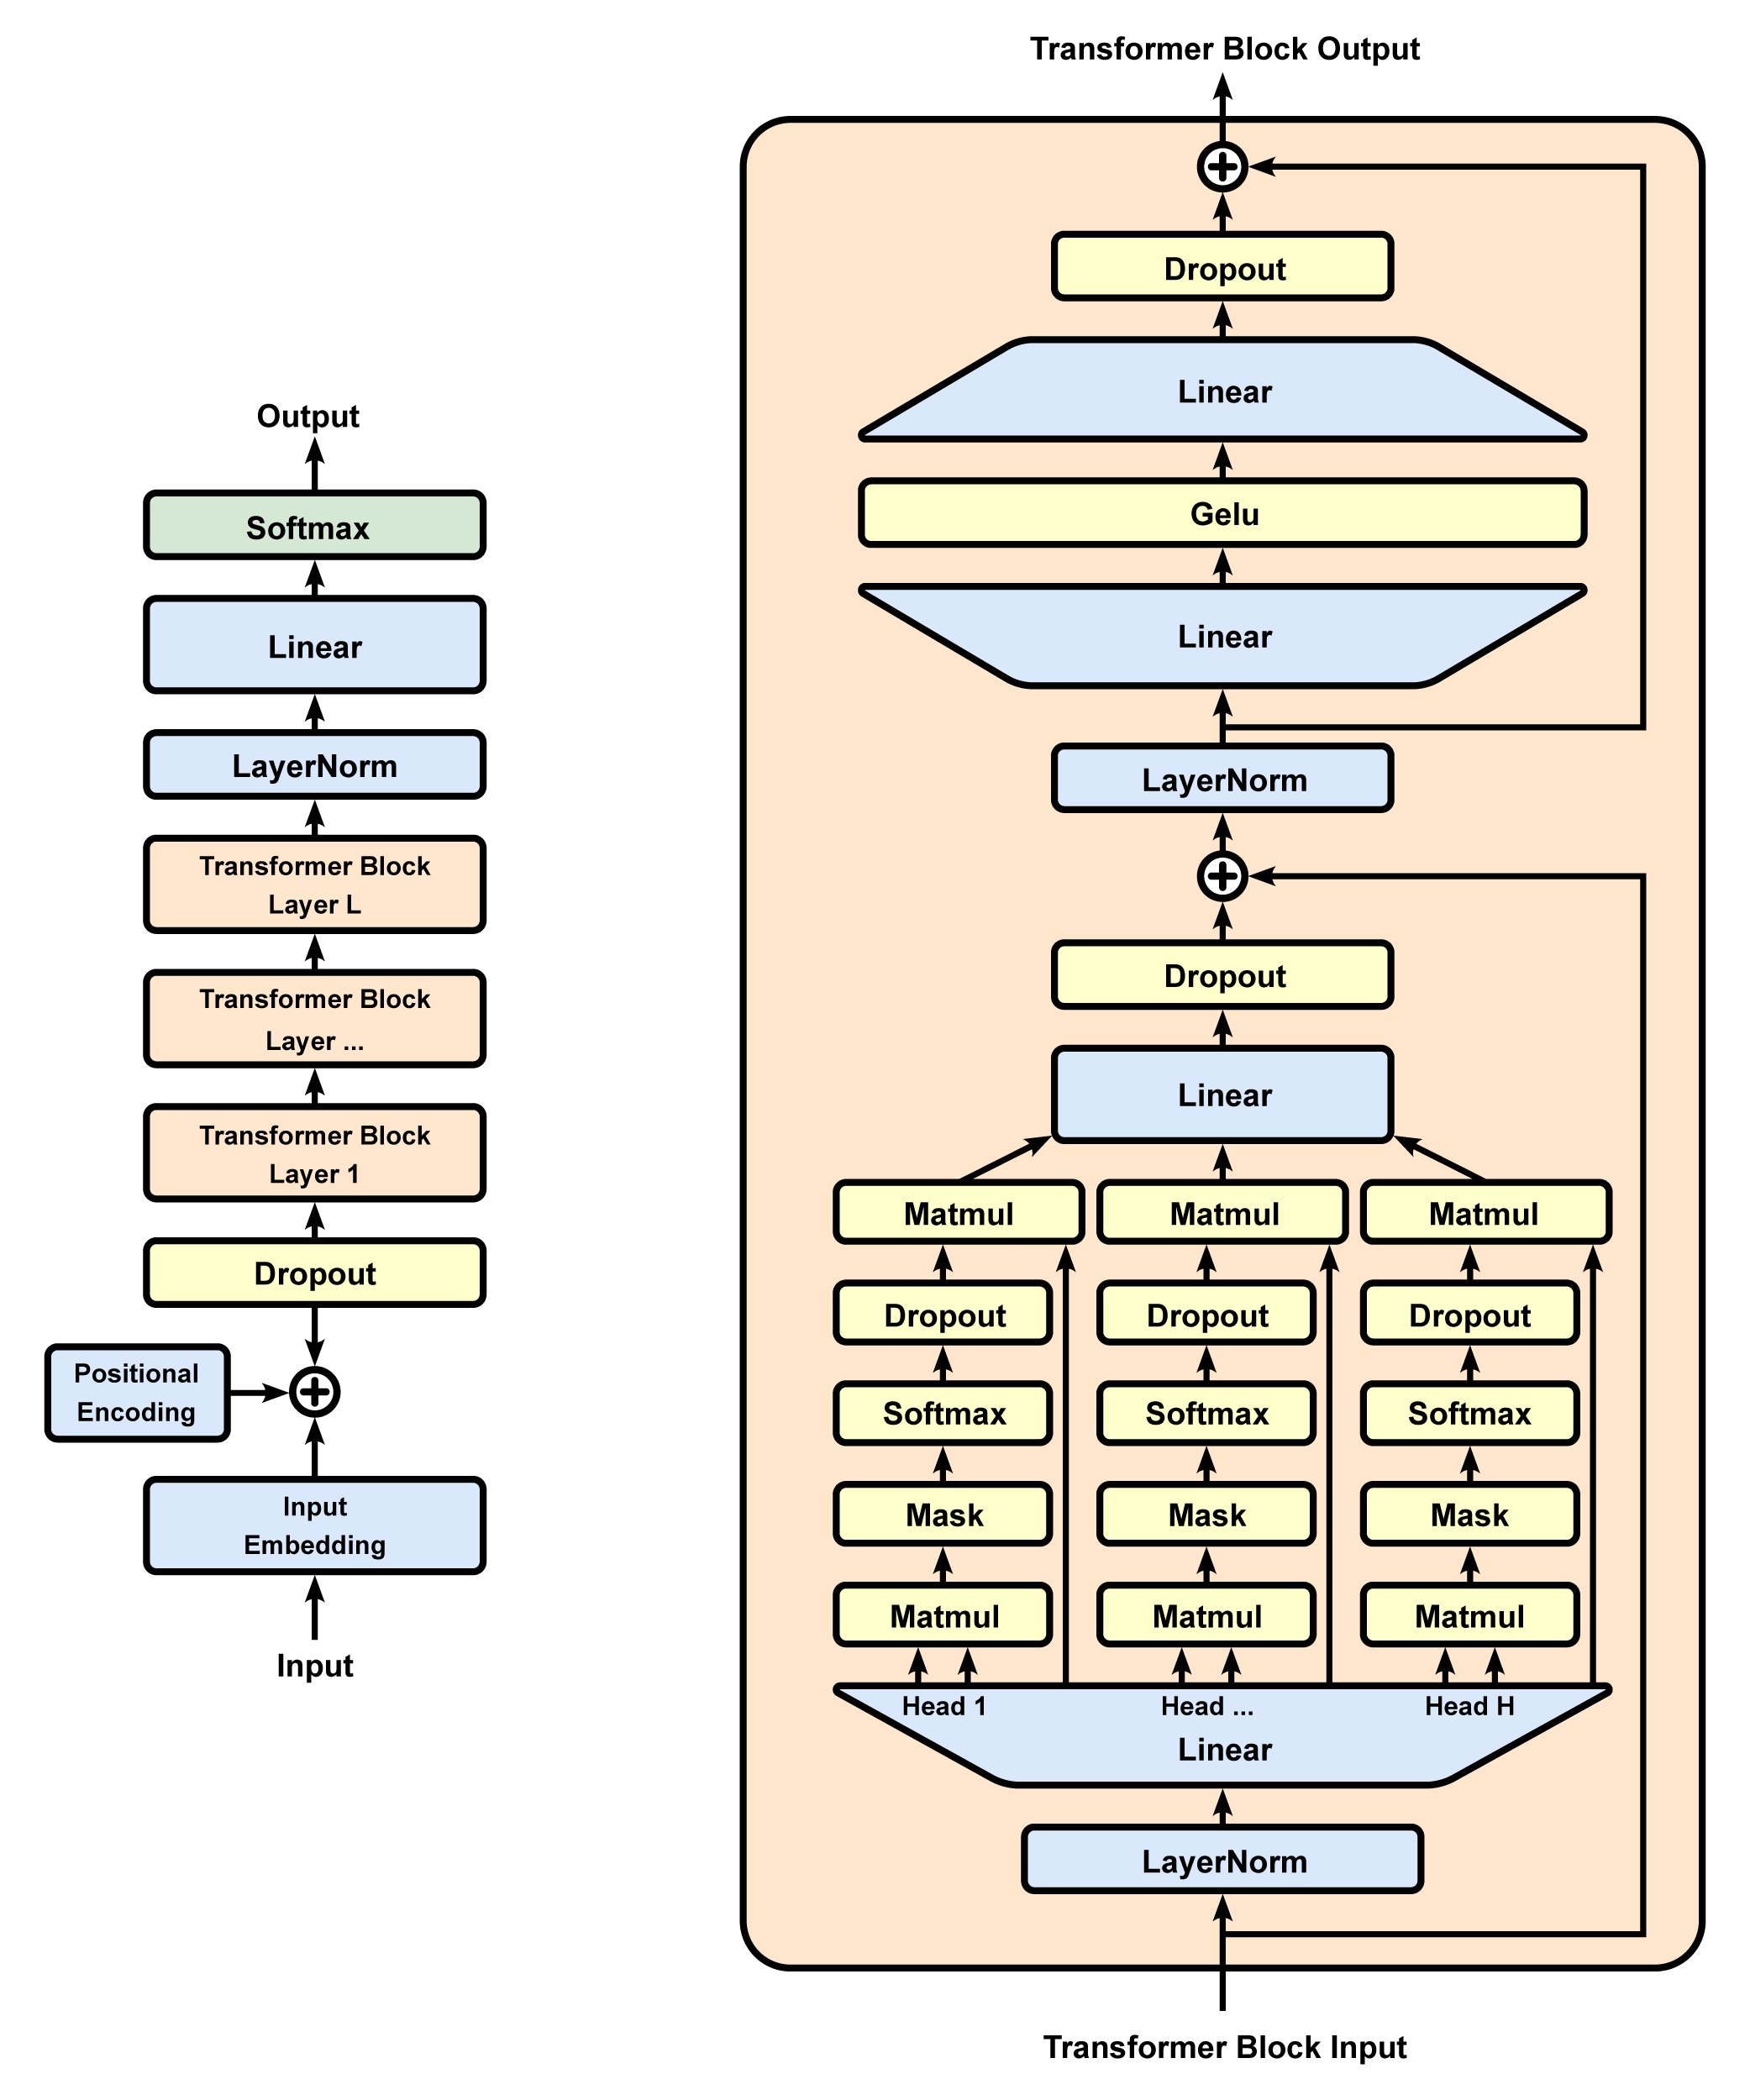
\includegraphics[width=1.0\linewidth]{figures/Full_GPT_architecture}
	\caption[Transformer Architecture]{The GPT Architecture~\cite{brown2020_language}}
	\label{fig:GPT_Architecture}
\end{figure}

In 2020 Facebook AI Research published a paper on Retrieval-Augmented Generation (RAG) which introduces an approach that combines the generative capabilities of models like GPT with the retrieval of factual information during the generation process~\cite{lewis2020retrieval}. This methodology enhances the model's ability to produce relevant and accurate responses by dynamically retrieving context from a vast corpus of data, representing a significant advancement in efforts to bridge the gap between human-like understanding and AI output.  Some examples of RAG models include:
\begin{enumerate}
	\item \textit{Call centre agent support}. Call centre agents require extensive knowledge of potentially hundreds of products and services, as well as commonly occurring product issues and their resolution. RAG solutions could assist agents in quickly finding answers to client requests.
	\item \textit{Customer chatbots}. RAG is strong enabler for creating customer-facing chatbots to answer frequently asked questions. Combining the natural language abilities of LLMs and the enterprise-specific responses of RAG can deliver a compelling, conversational customer experience.  
	\item \textit{Support / helpdesk}. Similar to call centre agents, IT operations and support personnel require deep knowledge of the configuration of complex systems deployments along with knowledge of common and previously seen issues and their resolution. RAG solutions could assist support personnel with quickly finding relevant answers to reported problems and observed issues.
\end{enumerate}

In the context of education, RAG offers transformative potential for educational environments by enhancing personalization, efficiency, and interaction in learning processes. By combining the generative capabilities of models like GPT with dynamic information retrieval, RAG can create tailored educational content, support research and writing, and enhance interactive tutoring systems~\cite{lewis2020retrieval}.  RAG's ability to pull relevant data from extensive knowledge bases allows it to generate accurate, context-specific content, making it ideal for developing personalized learning materials and dynamic assessment tools. Additionally, its application in question-answering systems can provide students with precise and informative responses, thereby fostering a deeper understanding of the subject matter~\cite{lewis2020retrieval}.

However, the integration of RAG into educational tools must be approached with caution, addressing potential challenges such as ensuring the accuracy and reliability of content, mitigating data biases, and upholding stringent privacy standards. Continuous collaboration with educators, careful dataset curation, and rigorous testing are essential to leverage RAG's capabilities effectively while maintaining educational integrity and compliance~\cite{holmes2019_artificial}.


\subsection{ChatGPT in Education}
\label{subsec:chatgpt_education}

ChatGPT, has been progressively integrated into educational contexts, showcasing potential across various teaching and learning activities. This section explores its primary applications and the emerging studies surrounding its efficacy and challenges in educational settings.

\subsubsection{Automated Content and Assessment Tools}
ChatGPT excels in generating and customizing educational content such as quizzes, reading materials, and assignments. It also offers potential in preliminary assessments by providing feedback on written assignments, which can be particularly beneficial in managing large classes~\cite{automated_content_generation}.

\subsubsection{Tutoring and Support}
As an interactive tutor, ChatGPT responds to student inquiries, assists with homework, and explains complex concepts, offering personalized support outside traditional classroom settings. This 24/7 availability can significantly enhance student learning, especially in subjects requiring frequent practice or clarification, such as languages and sciences~\cite{interactive_tutoring}.

\subsubsection{Enhancing Engagement and Language Learning}
In discussions, ChatGPT can stimulate engagement by posing challenging questions or introducing diverse viewpoints. For language learners, it serves as an invaluable practice tool, facilitating conversation in various languages, which helps improve linguistic fluency and cultural awareness~\cite{language_learning}.

\subsubsection{Challenges and Ethical Considerations}
Despite its benefits, the deployment of ChatGPT raises concerns regarding reliability, potential biases, and academic integrity. Misinformation, inherent biases from training data, and the potential for students to misuse essay-writing capabilities require careful consideration and regulation. Ensuring that these tools are used to complement traditional educational methods rather than replace them is crucial for maintaining the quality and integrity of education~\cite{chatgpt_challenges}.

The integration of these advanced Generative AI technologies in educational settings offers unprecedented opportunities for enhancing teaching and learning. Educators are leveraging these tools to develop more engaging and interactive learning environments, tailor educational content to individual needs, and foster critical thinking skills~\cite{holmes2019_artificial}. However, this integration also poses challenges, including ensuring the ethical use of AI in classrooms, protecting student data privacy, and maintaining academic integrity.

\subsection{Readability Metrics}
The following set of established readability metrics are important in the assessment of text difficulty, engagement, and appropriateness for educational content. 

\subsubsection{Readability Metrics Used in Educational Assessments}
Understanding the readability of educational content is crucial for tailoring materials to appropriate comprehension levels. This study employs several established readability metrics to evaluate the text complexity and accessibility of student-generated critiques. Below is a detailed explanation of each metric and its significance:

\begin{enumerate}	
	\item \textit{Flesch-Kincaid Grade Level}: Estimates the U.S. school grade level needed to understand the text. Lower scores indicate easier readability. A score of 12.0, for instance, suggests that the text is suitable for twelfth graders or equivalent~\cite{Farr_1951}. The Flesch-Kincaid grade level is calculated with the following formula: 
	
	{\footnotesize
		\begin{equation}
			0.39 \left(\frac{\text{total words}}{\text{total sentences}}\right) + 11.8 \left(\frac{\text{total syllables}}{\text{total words}}\right) - 15.59
		\end{equation}
	}
	
	\item \textit{Flesch Reading Ease}: Evaluates text simplicity based on the average sentence length and the average number of syllables per word. Scores range from 0 to 100, with higher scores indicating easier readability. For example, texts scoring between 60 and 70 are considered suitable for standard reading, while a score in the range of 10.0 - 30.0 is ranked at the `College graduate' level, typically very difficult to read and best understood by university graduates~\cite{Flesch_1948}. The Flesch Reading Ease score is calculated as follows: 

	{\footnotesize
		\begin{equation}
			\label{Flesch Reading Ease}
			206.835 - 1.015\left(\frac{\text{total words}}{\text{total sentences}}\right) - 84.6 \left(\frac{\text{total syllables}}{\text{total words}}\right)
		\end{equation}
	}

	\item \textit{Dale-Chall Readability Score}: Uses a list of familiar words to assess the grade level. Higher scores indicate more challenging text. A score of 9.0-10.0 suggests that the text is best understood by college-level readers~\cite{Dale_1948_DaleChall}. The Dale-Chall readability score is calculated with the following formula: 
	
	{\footnotesize
	\begin{equation}
		0.1579 \left(\frac{\text{difficult words}}{\text{words}} \times 100\right) + 0.0496 \left(\frac{\text{words}}{\text{sentences}}\right)
	\end{equation}
	}
	\item \textit{Automated Readability Index (ARI)}: Uses characters per word and words per sentence to estimate the grade level required for comprehension. A score of 13.0 indicates that the text is suitable for college freshmen~\cite{Senter_1971_ARI}. The ARI score is calculated: 
	
	\begin{equation}
		4.71 \left(\frac{\text{characters}}{\text{words}}\right) + 0.5 \left(\frac{\text{words}}{\text{sentences}}\right)
	\end{equation}
	
	\item \textit{Coleman Liau Index}: Estimates the U.S. school grade level necessary to understand the text, based on characters per word and words per sentence. A score of 11.0-12.0 indicates high school senior level complexity~\cite{Coleman_1975}. The Coleman–Liau index is calculated with the following formula:
	
	\begin{equation}
		CLI = 0.0588 \cdot L - 0.296 \cdot S - 15.8
	\end{equation}
	where $L$ is the average number of letters per 100 words and $S$ is the average number of sentences per 100 words.
	 
	\item \textit{Gunning Fog Index}: Estimates the years of formal education needed to understand the text. A score of 16.0 suggests college graduate level difficulty~\cite{Gunning_1952}. The Index is calculated as:
	
	\begin{equation}
		0.4 \left[\left(\frac{\text{words}}{\text{sentences}}\right) + 100 \left(\frac{\text{complex words}}{\text{words}}\right)\right]
	\end{equation}
	
	\item \textit{Linsear Write Formula}: Calculates the U.S. grade level based on sentence length and the number of easy or difficult words. A score of 8.0 means the text is suitable for eighth graders~\cite{Klare_1974}.  (See~\cite{Klare_1974} for the algorithm to compute the Linsear Write value.)
	
	\item \textit{SMOG Index (Simple Measure of Gobbledygook)}: Estimates the years of education needed to understand a text based on the number of polysyllabic words. A score of 17.0 implies graduate-level readability~\cite{McLaughlin_1969_SMOG}. SMOG is calculated using this formula:
	{\footnotesize
		\begin{equation}
			1.043 \sqrt{\text{num of polysyllables} \times \frac{30}{\text{num of sentences}}} + 3.1291
		\end{equation}
	}
	
	\item \textit{SPACHE Score}: Specifically designed for early readers, assessing sentence length and word familiarity. A score suitable for first to third graders would typically be below 4.0~\cite{Spache_1953}.  This instrument is not suitable for upper level undergraduate or graduate students.
\end{enumerate}

These readability metrics collectively provide insights into the accessibility of written content, ensuring that educational materials are appropriately challenging yet understandable for the intended audience.

\subsubsection{Additional Readability and Quality Metrics}
Beyond traditional readability metrics like the Flesch Reading Ease and Linsear Write Scores, other computational assessments such as the Bilingual Evaluation Understudy (BLEU), Recall-Oriented Understudy for Gisting Evaluation (ROUGE), and Metric for Evaluation of Translation with Explicit Ordering (METEOR) provide a broader evaluation of text quality, especially in contexts involving generative AI. BLEU measures the precision of generated text against reference texts by comparing the overlap of phrases and their order, making it ideal for assessing translation accuracy and content generation tasks in educational tools. This metric is widely used in machine translation to quantify how closely machine-generated text resembles human-like translations. Similarly, ROUGE is crucial for evaluating the coverage and recall of summaries produced by AI, ensuring that essential content is not omitted. It compares the extent to which the generated summaries capture the content present in a set of reference summaries, which is particularly useful in the evaluation of text summarization systems. Meanwhile, METEOR enhances evaluation by incorporating synonymy and stemming, alongside exact word matching, providing a balanced measure of fluency and intent preservation in generated text. Unlike BLEU, METEOR is designed to align more closely with human judgment by accounting for the flexibility in language use. Collectively, these metrics help in assessing the suitability of AI-generated educational content, aligning it with pedagogical goals and learner needs. Their application ensures that educational tools powered by AI not only generate content that is factually accurate but also presented in a manner that is understandable and engaging for students.

In summary, both BLEU and METEOR are traditionally utilized in machine translation to evaluate the alignment of translated text against one or more reference texts. These metrics quantify the extent of word and phrase overlap in the machine-generated text relative to the reference texts. Meanwhile, ROUGE assesses the quality of summaries by measuring the overlap between a generated summary and reference summaries, focusing particularly on the recall of essential content. However, in this study, there are no \textit{reference texts} available that would typically be required for these metrics to function effectively. Consequently, traditional readability metrics, which do not rely on reference texts, are deemed most appropriate for evaluating the critiques created by the students.

In the next section, we present the methodology supporting our investigation into the potential of LLMs to bolster students' critical thinking and writing capabilities.
\section{Methodology}
\label{Methodology}

\documentclass{article}
\usepackage{graphicx} % Required for inserting images
\graphicspath{ {./Figures/} }
\usepackage[rightcaption]{sidecap}
\usepackage[table]{xcolor}
\usepackage{multirow}
\usepackage{wrapfig}
\usepackage{makecell}

\begin{document}

\section{Findings}
\label{Findings}

\subsection{JSoup Library}
\vspace{0.3cm}
\centerline{Figure 1: Test Execution Time Against Number of Containers for JSoup Library (Scaling Memory)}
\vspace{0.3cm}
\centerline{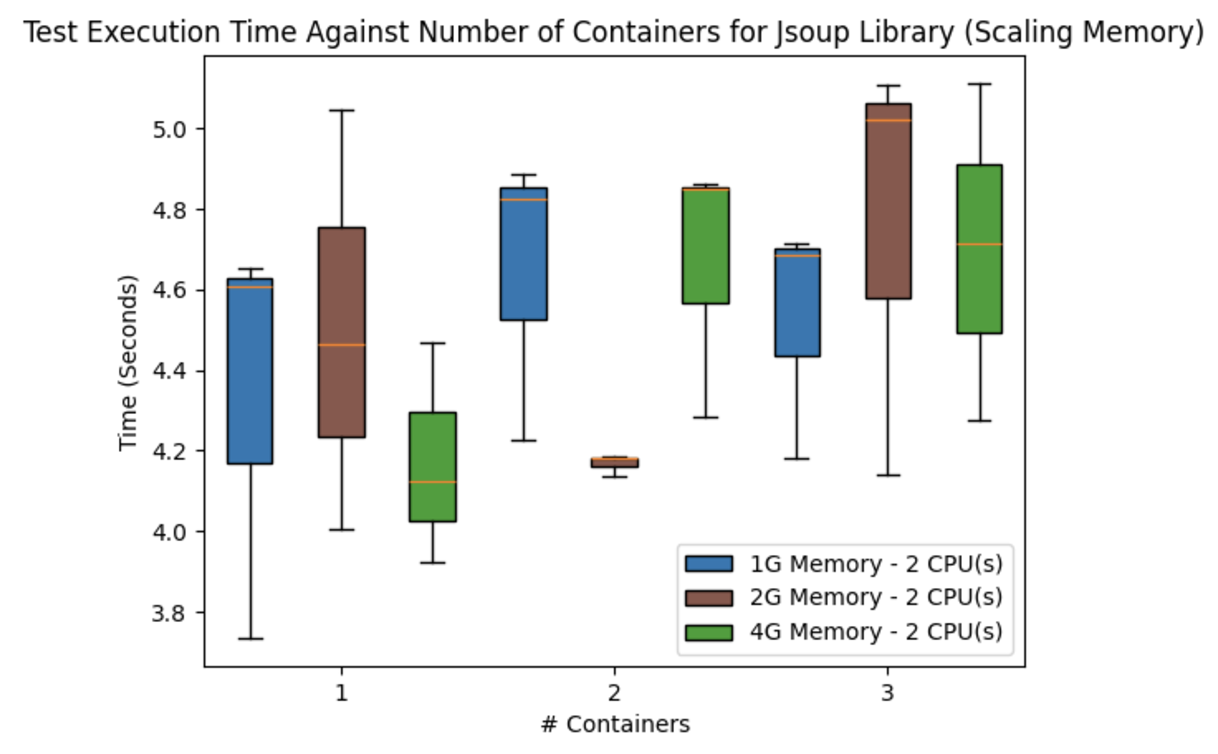
\includegraphics[width=12cm]{Figure1}}

\noindent{Figure 1 displays an insignificant improvement in test execution time as the number of containers increases. For each configuration, a one-way ANOVA test is performed to investigate if the difference in the mean execution time is statistically significant when the number of containers is increased. This indicates no evidence to suggest a difference in test execution time. The following configurations were used:}

\centerline{Table 1} 
\vspace{0.3cm}
{\centering
\begin{tabular}{|c|c|c|}
\rowcolor{gray!30}
    \hline
    Configuration & Significance (p value) & p \texttt{<} 0.05 \\
    \hline
     1G Memory – 2 CPUs & 0.6503 & No \\
     2G Memory – 2 CPUs & 0.3166 & No \\
     4G Memory – 2 CPUs & 0.1951 & No \\
     \hline
\end{tabular}
\par}

\vspace{0.4cm}
\noindent{Figure 1 also does not show a significant difference when increasing the amount of memory. Performing one-way ANOVA tests between configurations shows no statistically significant difference in the mean test execution time, regardless of the number of containers.} 

\centerline{Table 2} 
\vspace{0.3cm}
{\centering
\begin{tabular}{|c|c|c|}
\rowcolor{gray!30}
    \hline
    Container Number & Significance (p value) & p \texttt{<} 0.05 \\
    \hline
     1 & 0.6838 & No \\
     2 & 0.1284 & No \\
     3 & 0.7994 & No \\
     \hline
\end{tabular}
\par}

\newpage
\centerline{Figure 2: Test Execution Time Against Number of Containers for JSoup Library (Scaling CPUs)}
\vspace{0.3cm}
\centerline{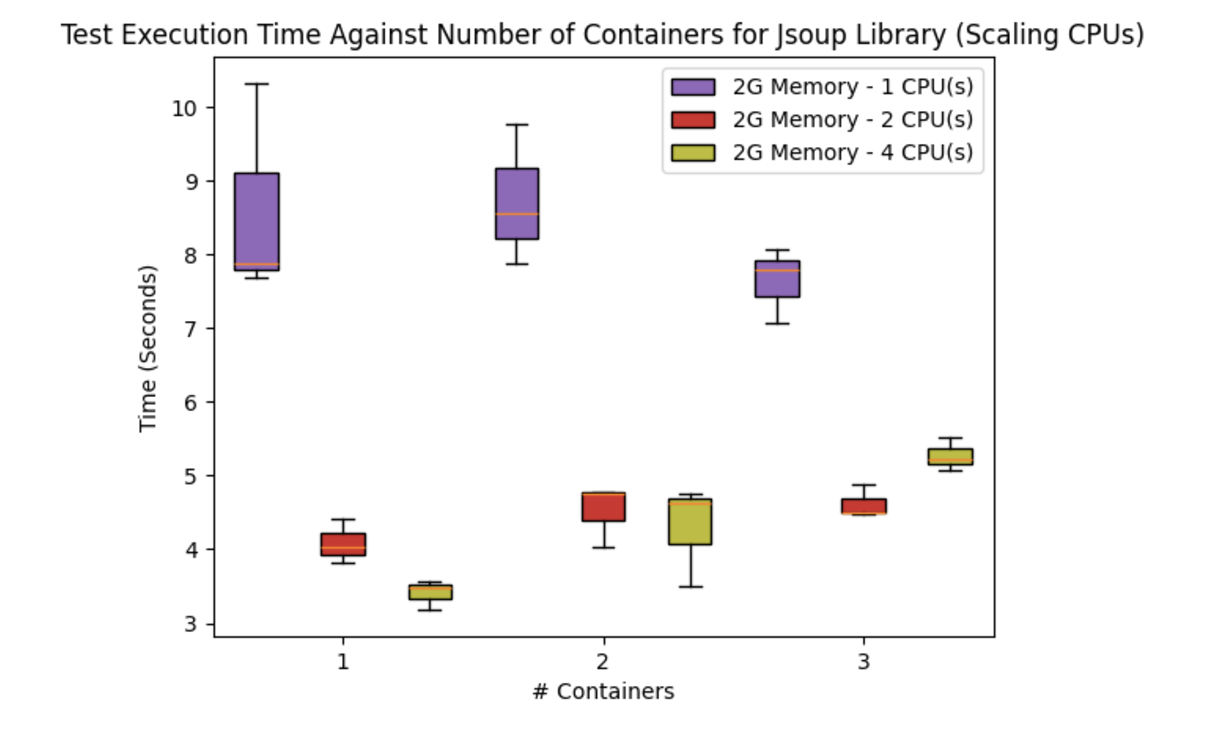
\includegraphics[width=12cm]{Figure2}}

\noindent{Figure 2 displays mixed results. When testing 2G Memory – 1 CPU, a slight improvement at 3 containers is observed, while testing 2G Memory – 2 CPUs and 2G Memory – 4 CPUs by increasing the number of containers seems to increase the test execution time. For each configuration, a one-way ANOVA test is performed to investigate if the difference in the mean execution time is statistically significant when increasing the number of containers. For scaling container CPUs, no evidence was found to suggest a difference in the test execution times, with exceptions to 2G Memory – 4 CPUs which had a p value of 0.0056.}

\centerline{Table 3} 
\vspace{0.3cm}
{\centering
\begin{tabular}{|c|c|c|}
\rowcolor{gray!30}
    \hline
    Configuration & Significance (p value) & p \texttt{<} 0.05 \\
    \hline
     2G Memory – 1 CPU & 0.4321 & No \\
     2G Memory – 2 CPUs & 0.1885 & No \\
     2G Memory – 4 CPUs & 0.0056 & Yes \\
     \hline
\end{tabular}
\par}

\vspace{0.4cm}
\noindent{Upon further investigating 2G Memory – 4 CPUs, the results suggest that increasing the number of containers increased test execution time. Performing right-tailed two-sample t-tests verified that the mean execution times increased as the number of containers increased.}

\vspace{0.2cm}
\centerline{Table 4} 
\vspace{0.3cm}
{\centering
\begin{tabular}{|c|c|c|}
\rowcolor{gray!30}
    \hline
    Container Testing & Significance (p value) & p \texttt{<} 0.05 \\
    \hline
     2 containers slower than 1 container & 0.0488 & Yes \\
     3 Containers slower than 1 Container & 0.0002 & Yes \\
     3 Containers slower than 2 Containers & 0.0402 & Yes \\
     \hline
\end{tabular}
\par}

\vspace{0.4cm}
\noindent{Figure 2 also shows some indication that increasing the number of CPUs decreased the execution time. To investigate further, one-way ANOVA tests were performed between configurations at each number of containers. This showed some statistical evidence to suggest that the mean execution times differed based on the configuration.}


\centerline{Table 5} 
\vspace{0.3cm}
{\centering
\begin{tabular}{|c|c|c|}
\rowcolor{gray!30}
    \hline
    Number of Containers & Significance (p value) & p \texttt{<} 0.05 \\
    \hline
     1 & 0.0006 & Yes \\
     2 & 0.0005 & Yes \\
     3 & 8.830e-5 & Yes \\
     \hline
\end{tabular}
\par}

\vspace{0.4cm}
\noindent{A left-tailed two-sample t-tests is performed to determine if there is a statistically significant decrease in the execution times with CPU scaling. In general, these results demonstrate that increasing the number of CPUs results in a decrease in the test execution times. However, at 2 containers and 3 containers, there is no significant decrease in test execution times when scaling from 2 to 4 CPUs with p values of 0.3268 and 0.9886, respectively. Moreover, in the case of 3 containers, a significant increase in test execution times with a p value of 0.0114 can be observed.}

\centerline{Table 6} 
\vspace{0.3cm}
{\centering
\begin{tabular}{|c|c|c|c|}
\rowcolor{gray!30}
    \hline
     Number of Containers & Comparison & Significance (p value) & p \texttt{<} 0.05 \\
     \hline
     \multirow{3}{*}{1} & \multicolumn{1}{|c|}{2 CPUs faster than 1 CPU} & \multicolumn{1}{c|}                    {0.0032} & \multicolumn{1}{c|}{Yes} \\\cline{2-4}
                        & \multicolumn{1}{|c|}{4 CPUs faster than 1 CPU} & \multicolumn{1}{c|}{0.0018} & \multicolumn{1}{c|}{Yes} \\\cline{2-4}
                        & \multicolumn{1}{|c|}{4 CPUs faster than 2 CPUs} & \multicolumn{1}{c|}{0.0151} & \multicolumn{1}{c|}{Yes} \\\Xhline{1pt} 

    \multirow{3}{*}{2} & \multicolumn{1}{|c|}{2 CPUs faster than 1 CPU} & \multicolumn{1}{c|}                      {0.0012} & \multicolumn{1}{c|}{Yes} \\\cline{2-4}
                        & \multicolumn{1}{|c|}{4 CPUs faster than 1 CPU} & \multicolumn{1}{c|}{0.0015} & \multicolumn{1}{c|}{Yes} \\\cline{2-4}
                        & \multicolumn{1}{|c|}{4 CPUs faster than 2 CPUs} & \multicolumn{1}{c|}{0.3268} & \multicolumn{1}{c|}{No} \\\Xhline{1pt} 

    \multirow{3}{*}{3} & \multicolumn{1}{|c|}{2 CPUs faster than 1 CPU} & \multicolumn{1}{c|}                      {0.0003} & \multicolumn{1}{c|}{Yes} \\\cline{2-4}
                        & \multicolumn{1}{|c|}{4 CPUs faster than 1 CPU} & \multicolumn{1}{c|}{0.0009} & \multicolumn{1}{c|}{Yes} \\\cline{2-4}
                        & \multicolumn{1}{|c|}{4 CPUs faster than 2 CPUs} & \multicolumn{1}{c|}{0.9886} & \multicolumn{1}{c|}{No} \\\hline
\end{tabular}
\par}

\newpage
\subsection{Guava Library}
\vspace{0.3cm}
\centerline{Figure 3: Test Execution Time Against Number of Containers for Guava Library (Scaling Memory)}
\vspace{0.3cm}
\centerline{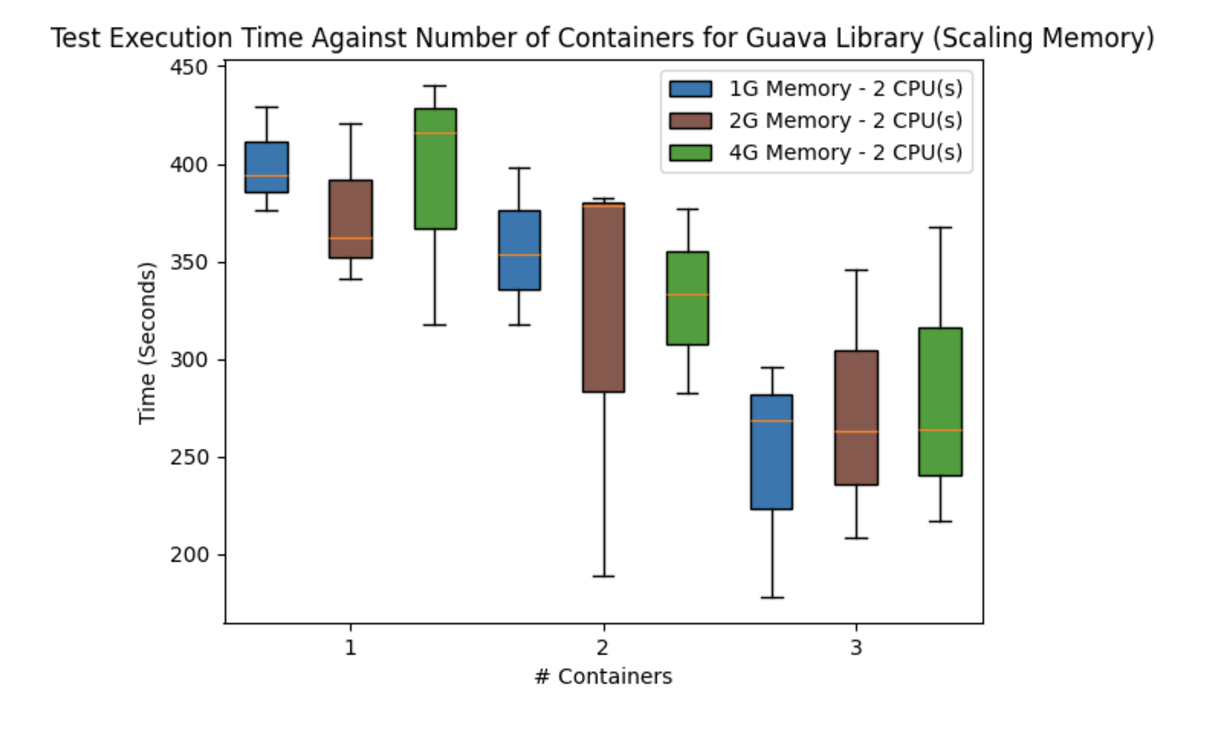
\includegraphics[width=12cm]{Figure3}}

\noindent{Figure 3 displays a downward trend as the number of containers increases. To verify this observation, one-way ANOVA tests are performed to determine the significance of the differences in test execution time as the number of containers increased.}

\centerline{Table 7} 
\vspace{0.3cm}
{\centering
\begin{tabular}{|c|c|c|}
\rowcolor{gray!30}
    \hline
    Configuration & Significance (p value) & p \texttt{<} 0.05 \\
    \hline
     1G Memory – 2 CPUs & 0.0154 & Yes \\
     2G Memory – 2 CPUs & 0.3463 & No \\
     4G Memory – 2 CPUs & 0.1977 & No \\
     \hline
\end{tabular}
\par}

\vspace{0.4cm}
\noindent{It was determined that only in the case of 1G Memory – 2 CPUs, is there a statistically significant difference when the number of containers is increased. To further investigate these differences, left-tailed two-sample t-tests are performed to determine the significance of the changes when increasing the number of containers. No significant decrease in test execution times was found when moving from 1 container to 2 containers, however, when moving from 1 container to 3 containers and 2 containers to 3 containers, there was a significant decrease with p values of 0.0085 and 0.0311 respectively.}

\newpage
\centerline{Table 8} 
\vspace{0.3cm}
{\centering
\begin{tabular}{|c|c|c|}
\rowcolor{gray!30}
    \hline
    Comparison & Significance (p value) & p \texttt{<} 0.05 \\
    \hline
     2 containers faster than 1 container & 0.0970 & No \\
     3 containers faster than 1 container & 0.0085 & Yes \\
     3 containers faster than 2 containers & 0.0311 & Yes \\
     \hline
\end{tabular}
\par}

\vspace{0.4cm}
\noindent{Figure 3, much like Figure 1, shows insignificant evidence that increasing the amount of memory reduced test execution times. One-way ANOVA tests were performed to determine if there was any statistically significant difference in test executions times. No evidence was found suggesting increasing memory improved test execution times regardless of the number of containers.}

\vspace{0.2cm}
\centerline{Table 9} 
\vspace{0.3cm}
{\centering
\begin{tabular}{|c|c|c|}
\rowcolor{gray!30}
    \hline
    Number of Containers & Significance (p value) & p \texttt{<} 0.05 \\
    \hline
     1 & 0.8061 & No \\
     2 & 0.8027 & No \\
     3 & 0.8180 & No \\
     \hline
\end{tabular}
\par}

\vspace{0.4cm}
\centerline{Figure 4: Test Execution Time Against Number of Containers for Guava Library (Scaling CPUs)}
\vspace{0.3cm}
\centerline{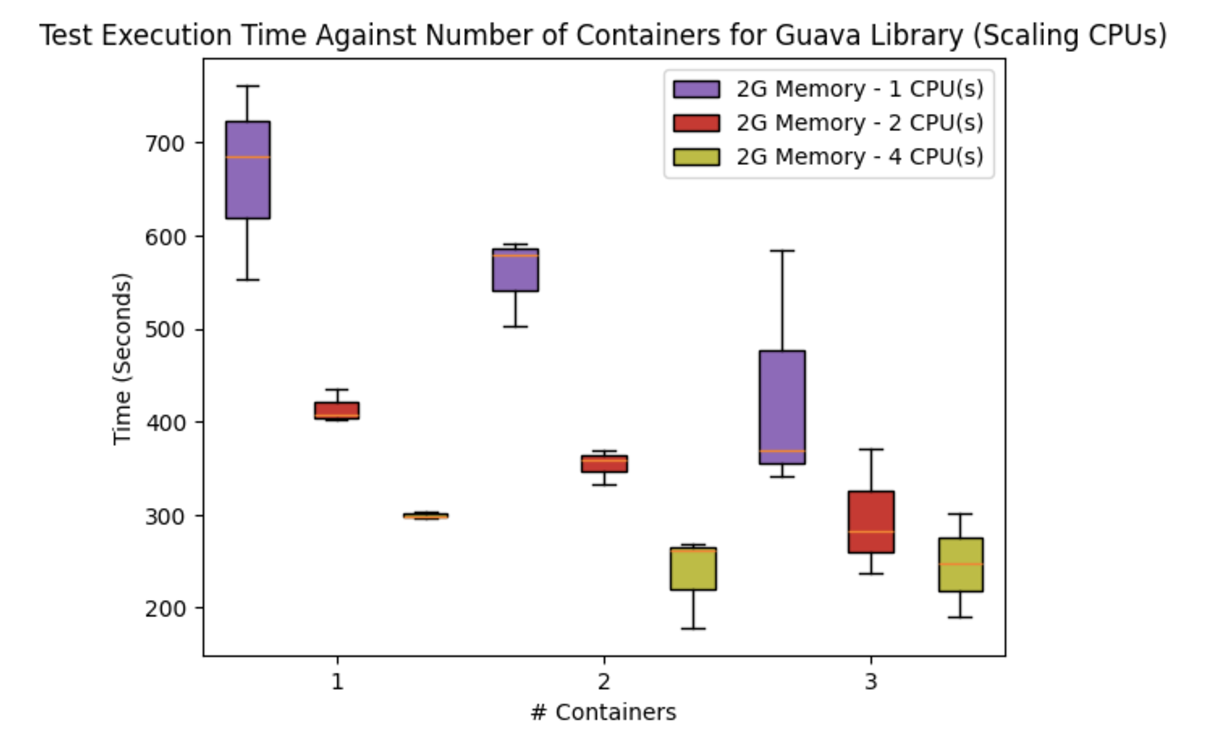
\includegraphics[width=12cm]{Figure4}}

\noindent{Figure 4 displays some significant decrease in the execution times. One-way ANOVA tests were performed to determine the significance of the differences in execution times as the number of containers increased for each configuration. Only significant differences for 2G Memory and 2 CPUs have been observed.}

\newpage
\centerline{Table 10} 
\vspace{0.3cm}
{\centering
\begin{tabular}{|c|c|c|}
\rowcolor{gray!30}
    \hline
    Configuration & Significance (p value) & p \texttt{<} 0.05 \\
    \hline
     2G Memory – 1 CPU & 0.0781 & No \\
     2G Memory – 2 CPUs & 0.0372 & Yes \\
     2G Memory – 4 CPUs & 0.2405 & No \\
     \hline
\end{tabular}
\par}

\vspace{0.4cm}
\noindent{To further investigate the differences found at 2G Memory and 2 CPUs, left-tailed two-sample t-tests were performed to determine if there was a presence of statistically significant decreases in test execution time as the number of containers increased. The results showcase that increasing from 1 container to 2 or 3 containers produces improved execution times with p values of 0.0075 and 0.0215, but not when increasing from 2 to 3 containers with a p value of 0.1158.}

\centerline{Table 11} 
\vspace{0.3cm}
{\centering
\begin{tabular}{|c|c|c|}
\rowcolor{gray!30}
    \hline
    Comparison & Significance (p value) & p \texttt{<} 0.05 \\
    \hline
     2 containers faster than 1 container & 0.0075 & Yes \\
     3 containers faster than 1 container & 0.0215 & Yes \\
     3 containers faster than 2 containers & 0.1158 & No \\
     \hline
\end{tabular}
\par}

\vspace{0.4cm}
\noindent{Additionally, Figure 4 shows that regardless of the number of containers, the test execution time can be improved by increasing the number of CPUs. One-way ANOVA tests were performed for each number of containers to determine any significant differences in test execution times. At 1 and 2 containers, the data suggests that increasing the number of CPUs had an impact on the execution time, with p values of 0.0009 and 0.0002, respectively. However, for 3 containers, no significant difference is observed.}

\vspace{0.2cm}
\centerline{Table 12} 
\vspace{0.3cm}
{\centering
\begin{tabular}{|c|c|c|}
\rowcolor{gray!30}
    \hline
    Number of Containers & Significance (p value) & p \texttt{<} 0.05 \\
    \hline
     1 & 0.0009 & Yes \\
     2 & 0.0002 & Yes \\
     3 & 0.1101 & No \\
     \hline
\end{tabular}
\par}

\vspace{0.4cm}
\noindent{To further investigate the differences found in test execution time for 1 and 2 containers, left-tailed two-sample t-tests were performed to determine the presence of significant decreases in test execution times as the number of CPUs increase. With both numbers of containers, the data suggests that increasing the number of CPUs results in lower test execution times.}

\newpage
\centerline{Table 13} 
\vspace{0.3cm}
{\centering
\begin{tabular}{|c|c|c|c|}
\rowcolor{gray!30}
    \hline
     Number of Containers & Comparison & Significance (p value) & p \texttt{<} 0.05 \\
     \hline
     \multirow{3}{*}{1} & \multicolumn{1}{|c|}{2 CPUs faster than 1 CPU} & \multicolumn{1}{c|}                    {0.0076} & \multicolumn{1}{c|}{Yes} \\\cline{2-4}
                        & \multicolumn{1}{|c|}{3 CPUs faster than 1 CPU} & \multicolumn{1}{c|}{0.0019} & \multicolumn{1}{c|}{Yes} \\\cline{2-4}
                        & \multicolumn{1}{|c|}{3 CPUs faster than 2 CPUs} & \multicolumn{1}{c|}{0.0002} & \multicolumn{1}{c|}{Yes} \\\Xhline{1pt} 

    \multirow{3}{*}{2} & \multicolumn{1}{|c|}{2 CPUs faster than 1 CPU} & \multicolumn{1}{c|}                      {0.0012} & \multicolumn{1}{c|}{Yes} \\\cline{2-4}
                        & \multicolumn{1}{|c|}{3 CPUs faster than 1 CPU} & \multicolumn{1}{c|}{0.0006} & \multicolumn{1}{c|}{Yes} \\\cline{2-4}
                        & \multicolumn{1}{|c|}{3 CPUs faster than 2 CPUs} & \multicolumn{1}{c|}{0.0096} & \multicolumn{1}{c|}{Yes} \\\Xhline{1pt} 
\end{tabular}
\par}

\end{document}

\section{Discussion}
\label{Discussion}

\section{Conclusion}
\label{Conclusion}

Replace all this with your Conclusion.  The Conclusion provides a concise summary of the main findings and their implications. It reinforces the key takeaways from the research, emphasizing the overall contribution to the field. The conclusion often includes final thoughts on the study’s significance, practical applications, and, if applicable, recommendations for future research. It should leave the reader with a clear understanding of the study’s value and outcomes without introducing new information.

This study explored the impact of integrating ChatGPT into academic critique writing, highlighting notable improvements in the writing quality and analytical depth across various metrics. The results affirm the potential of AI tools to not only enhance traditional educational methods but also to personalize and enrich learning experiences for both educators and students.

However, the study's limitations, including its small sample size and the demographic homogeneity of the participants, caution against broad generalizations of these findings. The short duration of the study also limits insights into the long-term effects of AI integration in educational settings. Future research should, therefore, expand these investigations across more diverse educational contexts and over longer periods to better understand the enduring impacts of AI on learning outcomes. It is also essential to address the ethical challenges associated with AI use in education, such as ensuring data privacy and managing the risk of academic dishonesty, through the development of robust ethical frameworks and guidelines.


\subsection{Future Research}
As AI continues to integrate into educational landscapes, it is imperative for educators, researchers, and policymakers to adopt a balanced approach to its use. This approach should aim to ensure that AI complements traditional teaching methodologies, enhancing educational outcomes while safeguarding the integrity and rigour of academic processes.

The sample size in this study was very small, comprising only 22 participants. Future work should include larger and more diverse samples to cross-validate the findings. Additionally, this study spanned only one semester; future research should consider extending the duration to several semesters or even academic years to assess the long-term effects on student learning outcomes. Conducting such longitudinal studies would yield a more comprehensive dataset.

Lastly, while this paper briefly addressed ethical questions about AI in education, further research is needed to elaborate on measures that could minimize potential biases and ensure academic integrity. Such efforts would pave the way for establishing practical guidelines for educators.
%
% ---- Bibliography ----
%
% BibTeX users should specify bibliography style 'splncs04'.
% References will then be sorted and formatted in the correct style.
%
%\bibliographystyle{plain} % or another style you're using
\bibliographystyle{splncs04}
\bibliography{bibliography}

\input{Appendix}

\end{document}
